\documentclass[10pt,a4paper]{ctexart}
\usepackage{wrapfig}
\usepackage{amsmath}
\usepackage{amsfonts}
\usepackage{amssymb}
\usepackage{graphicx}
\usepackage[left=3.18cm, right=3.18cm, top=2.56cm, bottom=2.56cm]{geometry}
\usepackage{ulem}
\setlength{\parindent}{2em}
\newcommand{\nianfen}[1]{\hspace{-2em}{(#1\textbf{·}\textit{青岛}\textbf{·}23)}}
\newcommand{\ckong}{\rule{14em}{0.5pt}}
\newcommand{\kong}{\rule{4em}{0.5pt}}
\begin{document}
	\nianfen{2017}数和形是数学的两个主要研究对象,我们经常运用数形结合、数形转化的方法解决一些数学问题.下面我们来探究“由数思形,以形助数”的方法在解决代数问题中的应用.
	
	\textbf{探究一:求不等式$|x-1|<2$的解集}
	
	(1)探究$|x-1|$的几何意义
	
	如图\textcircled{1},在以$O$为原点的数轴上,设点$ A' $对应的数是$x-1 $,由绝对值的定义可知,点$  A' $与点$ O  $的距离为$ |x-1| $,可记为 $ A'O=|x-1| $.将线段 $ A'O $ 向右平移$ 1 $个单位得到线段 $ AB $ ,此时点 $ A $ 对应的数是$x $ ,点 $ B $ 对应的数是$ 1 $.因为 $ AB= A'O $ ,所以 $ AB=|x-1| $ .因此,$ |x-1| $的几何意义可以理解为数轴上$x  $所对应的点$  A  $与$ 1 $所对应的点 $ B $ 之间的距离 $ AB $ .
	
	\begin{center}
		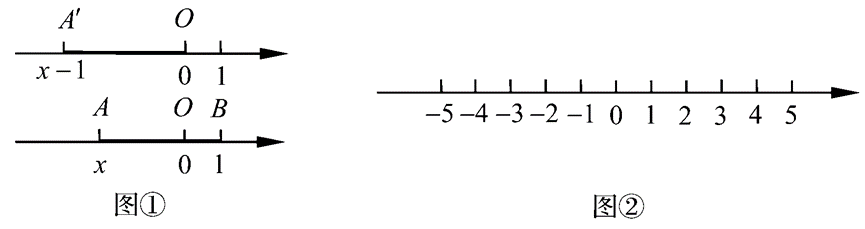
\includegraphics[width=0.8\linewidth]{D:/schoolmaterial/doc/MATH2324/23/2017a}
	\end{center}
	
	(2)求方程$ |x-1|=2 $ 的解
	因为数轴上3和-1所对应的点与1所对应的点之间的距离都为2 ,所以方程的解为3,-1.
	
	(3)求不等式$ |x-1|<2 $ 的解集
	因为$ |x-1| $表示数轴上$ x $ 所对应的点与1所对应的点之间的距离,所以求不等式解集就转
	化为求这个距离小于 2 的点对应的数$ x $ 的范围.
	请在图\textcircled{2}的数轴上表示$ |x-1|<2 $ 的解集,并写出这个解集\kong.
	
	\begin{center}
		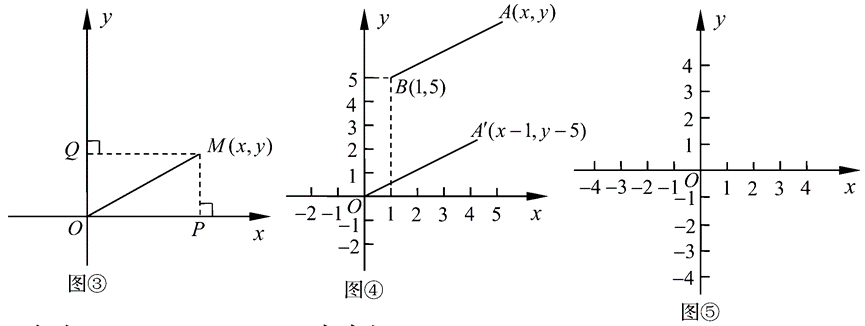
\includegraphics[width=0.9\linewidth]{23/2017b}
	\end{center}
	
	\textbf{探究二:探究 $ \sqrt{(x-a)^2+(y-b)^2} $ 的几何意义}
	
	(1)探究 $ \sqrt{x^2+y^2} $ 的几何意义
	
	如图\textcircled{3},在直角坐标系中,设点 $ M $ 的坐标为$ (x,y) $,过 $ M $ 作 $ MP\perp  x $ 轴于 $ P $ ,作 $ MQ\perp  y $
	轴于$ Q $ ,则 $ P $ 点坐标为$ (x,0) $,$ Q $ 点坐标为$ (0,y) $,$ OP=|x| $ ,$ OQ=|y| $,在 $ Rt\triangle  OPM $ 中,
	$ PM=OQ=|y| $,则 $ MO=\sqrt{OP^2+PM^2}=\sqrt{|x|^2+|y|^2}=\sqrt{x^2+y^2} $ .因此, $\sqrt{x^2+y^2}$ 的几何意义可以理解为点 $ M(x,y) $与点$ O(0,0) $之间的距离 $ MO $ .
	
	(2)探究 $\sqrt{(x-1)^2+(y-5)^2}$ 的几何意义
	
	如图\textcircled{4},在直角坐标系中,设点$  A' $ 的坐标为$ (x-1,y-5) $,由探究二(1)可知,
	$ A'O=\sqrt{(x-1)^2+(y-5)^2}$ .将线段 $ A'O $ 先向右平移 1 个单位,再向上平移 5 个单位,得到线段
	$ AB $ , 此 时 点 $ A $ 的 坐 标 为$  (x,y ) $, 点 $ B $ 的 坐 标 为 (1, 5). 因 为 $ AB=A'O $ , 所 以
	$AB=\sqrt{(x-1)^2+(y-5)^2}$ .因此, $\sqrt{(x-1)^2+(y-5)^2}$ 的几何意义可以理解为点 $ A(x,y) $与点
	$ B(1,5) $之间的距离 $ AB $ .
	
	(3)探究$\sqrt{(x+3)^2+(y-4)^2}$ 的几何意义
	
	请仿照探究二(2)的方法,在图\textcircled{5}中画出图形,并写出探究过程.
	
	\rule{0em}{3em}
	
	(4) $\sqrt{(x-a)^2+(y-b)^2}$ 的几何意义可以理解为:\ckong.
	
	\textbf{拓展应用:}
	
	(1) $\sqrt{(x-2)^2+(y+1)^2}+\sqrt{(x+1)^2+(y+5)^2}$ 的几何意义可以理解为:点$  A(x,y) $与点
	$ E (2,-1) $的距离和点 $ A(x,y) $与点 $ F $\kong (填写坐标)的距离之和.
	
	(2) $\sqrt{(x-2)^2+(y+1)^2}+\sqrt{(x+1)^2+(y+5)^2}$ 的最小值为\kong. (直接写出结果)
	
	\mbox{}
	
	\nianfen{2016}
	
	\textbf{问题提出:}如何将边长为 $ n(n\geq 5 $,且 $ n $ 为整数)的正方形分割为一些 1×5 或 2×3 的矩形
	($ a×b $ 的矩形指边长分别为 $ a,b $ 的矩形)?
	
	\textbf{问题探究:}我们先从简单的问题开始研究解决,再把复杂问题转化为已解决的问题.
	
	\textbf{探究一:}
	如图\textcircled{1},当 $ n=5 $ 时,可将正方形分割为五个 1×5 的矩形.
	如图\textcircled{2},当 $ n=6 $ 时,可将正方形分割为六个 2×3 的矩形.
	如图\textcircled{3},当 $ n=7 $ 时,可将正方形分割为五个 1×5 的矩形和四个 2×3 的矩形.
	如图\textcircled{4},当 $ n=8 $ 时,可将正方形分割为八个 1×5 的矩形和四个 2×3 的矩形.
	如图\textcircled{5},当 $ n=9 $ 时,可将正方形分割为九个 1×5 的矩形和六个 2×3 的矩形.
	
	\begin{center}
		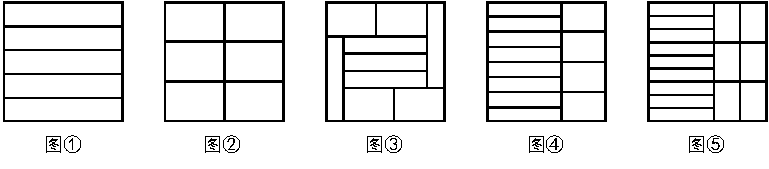
\includegraphics[width=0.9\linewidth]{23/2016a}
	\end{center}
	
	\textbf{探究二:}
	
	当 $ n=10,11,12,13,14 $ 时,分别将正方形按下列方式分割:
	
	\begin{center}
		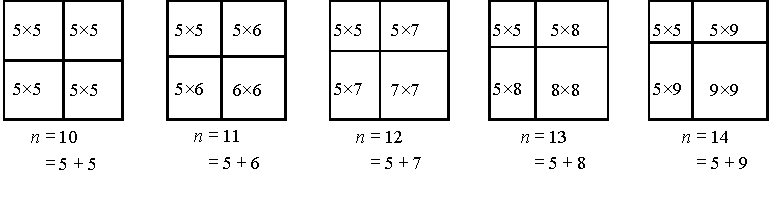
\includegraphics[width=0.9\linewidth]{23/2016b}
	\end{center}
	
	所以,当 $ n=10,11,12,13,14 $ 时,均可将正方形分割为一个 5×5 的正方形、一个
	$ (n-5)×(n-5) $的正方形和两个 $ 5×(n-5) $的矩形.显然, 5×5 的正方形和 $ 5×(n-5) $
	的矩形均可分割为 1×5 的矩形,而$ (n-5)×(n-5) $的正方形是边长分别为 5,6,7,8,9
	的正方形,用探究一的方法可分割为一些 1×5 或 2×3 的矩形.
	
	\textbf{探究三:}
	当 $ n=15,16,17,18,19 $ 时,分别将正方形按下列方式分割:
	
	\begin{center}
		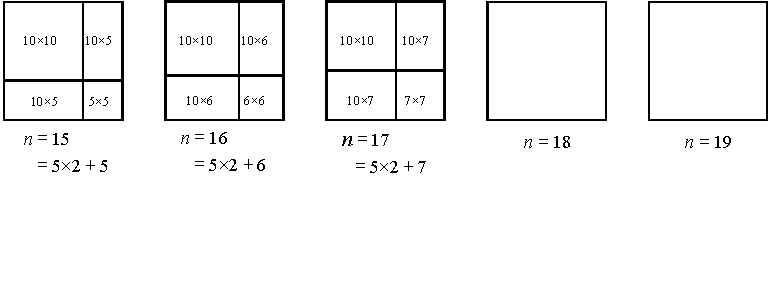
\includegraphics[width=0.9\linewidth]{23/2016c}
	\end{center}
	
	请按照上面的方法,分别画出边长为 18,19 的正方形分割示意图.
	
	所以,当 $ n=15,16,17,18,19 $ 时,均可将正方形分割为一个 10×10 的正方形、一个
	$ (n-10)×(n-10) $的正方形和两个 $ 10×(n-10) $的矩形.显然,10×10 的正方形和 $ 10×(n-10) $
	的矩形均可分割为 1×5 的矩形,而$ (n-10)×(n-10) $的正方形又是边长分别为 5,6,7,8,9 的正方形,用探究一的方法可分割为一些 1×5 或 2×3 的矩形.
	
	\textbf{问题解决:}如何将边长为 $ n(n\geq 5 $,且 $ n $ 为整数)的正方形分割为一些 1×5 或 2×3 的矩形?请按照上面的方法画出分割示意图,并加以说明.
	
	\rule{0em}{5em}
	
	\textbf{实际应用:}如何将边长为 61 的正方形分割为一些 1×5 或 2×3 的矩形?(只需按照探究三的方
	法画出分割示意图即可)
	
	\mbox{}
	
	\nianfen{2015}
	
	\textbf{问题提出:}用$ n $根相同的木棒搭一个三角形(木棒无剩余),能搭成多少种不同的等腰三角形?
	
	\textbf{问题探究:}不妨假设能搭成$ m $种不同的等腰三角形,为探究$ m $与$ n $之间的关系,我们可以先从特殊入手,通过试验、观察、类比、最后归纳、猜测得出结论. 
	
	\textbf{探究一:}
	
	(1)用3根相同的木棒搭一个三角形,能搭成多少种不同的等腰三角形?
	
	此时,显然能搭成一种等腰三角形.
	
	所以,当$ n=3 $时,$ m=1 $. 
	
	(2)用4根相同的木棒搭一个三角形,能搭成多少种不同的等腰三角形?
	
	只可分成1根木棒、1根木棒和2根木棒这一种情况,不能搭成三角形.
	
	所以,当$ n=4 $时,$ m=0 $. 
	
	(3)用5根相同的木棒搭一个三角形,能搭成多少种不同的等腰三角形?
	
	若分成1根木棒、1根木棒和3根木棒,则不能搭成三角形.
	
	若分成2根木棒、2根木棒和1根木棒,则能搭成一种等腰三角形.
	
	所以,当$ n=5 $时,$ m=1 $.
	
	(4)用6根相同的木棒搭一个三角形,能搭成多少种不同的等腰三角形?
	
	若分成1根木棒、1根木棒和4根木棒,则不能搭成三角形.
	
	若分成2根木棒、2根木棒和2根木棒,则能搭成一种等腰三角形.
	
	所以,当$ n=6 $时,$ m=1 $.
	
	综上所述,可得表\textcircled{1}:
	
	\begin{center}
		\begin{tabular}{|c|c|c|c|c|}
		\hline 
		$n$ & 3 & 4 & 5 & 6 \\ 
		\hline 
		$m$ & 1 & 0 & 1 & 1 \\ 
		\hline 
	\end{tabular} 
	\end{center}
	
	\textbf{探究二:}
	
	(1)用7根相同的木棒搭一个三角形,能搭成多少种不同的三角形? (仿照上述探究方法,写出解答过程,并将结果填在表\textcircled{2}中) 
	
	(2)用8根、9根、10根相同的木棒搭一个三角形,能搭成多少种不同的等腰三角形? (只需把结果填在表\textcircled{2}中)
	
	表\textcircled{2}:
	
	\begin{center}
		\begin{tabular}{|c|c|c|c|c|}
		\hline 
		$n$ & 7 & 8 & 9 & 10\\ 
		\hline 
		$m$ &  &  &  &  \\ 
		\hline 
	\end{tabular} 
	\end{center}
	
	你不妨分别用11根、12根、13根、14根相同的木棒继续进行探究…
	
	\textbf{问题解决:}用$ n $根相同的木棒搭一个三角形(木棒无剩余),能搭成多少种不同的等腰三角形?(设$ n $分别等于$ 4k-1 $,$ 4k $,$ 4k+1 $,$ 4k+2 $,其中$ k $是正整数,把结果填在表\textcircled{3}中) 
	
	表\textcircled{3}:
	
	\begin{center}
		\begin{tabular}{|c|c|c|c|c|}
		\hline 
		$n$ & $4k-1$ & $4k$ & $4k+1$ & $4k+2$\\ 
		\hline 
		$m$ &  &  &  &  \\ 
		\hline 
	\end{tabular}
	\end{center} 

	\textbf{问题应用:}用2016根相同的木棒搭一个三角形(木棒无剩余),能搭成多少种不同的等腰三角形?(写出解答过程),其中面积最大的等腰三角形每腰用了\kong 根木棒.(只填结果)
	
	\mbox{}
	
	\nianfen{2014}
	
	\textbf{数学问题:}计算${{\frac{{{1}}}{{{m}}}}{+}{\frac{{{1}}}{{{m}{^{{2}}}}}}{+}{\frac{{{1}}}{{{m}{^{{3}}}}}}{+}{\cdots 
		}{+}{\frac{{{1}}}{{{m}{^{{n}}}}}}}$(其中$m,n$都是正整数,且$m\ge 
	$2,$n\ge $1).
	
	\textbf{探究问题:}为解决上面的数学问题,我们运用数形结合的思想方法,通过不断地分割一个面积为1的正方形,把数量关系和几何图形巧妙地结合起来,并采取一般问题特殊化的策略来进行探究.
	
	\textbf{探究一:}计算${{\frac{{{1}}}{{{2}}}}{+}{\frac{{{1}}}{{{2}{^{{2}}}}}}{+}{\frac{{{1}}}{{{2}{^{{3}}}}}}{+}{\cdots 
		}{+}{\frac{{{1}}}{{{2}{^{{n}}}}}}}$.
	
	第1次分割,把正方形的面积二等分,其中阴影部分的面积为${{\frac{{{1}}}{{{2}}}}}$;
	
	第2次分割,把上次分割图中空白部分的面积继续二等分,阴影部分的面积之和为${{\frac{{{1}}}{{{2}}}}{+}{\frac{{{1}}}{{{2}{^{{2}}}}}}}$;
	
	第3次分割,把上次分割图中空白部分的面积继续二等分,{\ldots}{\ldots};
	
	{\ldots}{\ldots}
	
	第$n$次分割,把上次分割图中空白部分的面积最后二等分,所有阴影部分的面积之和
	
	为${{\frac{{{1}}}{{{2}}}}{+}{\frac{{{1}}}{{{2}{^{{2}}}}}}{+}{\frac{{{1}}}{{{2}{^{{3}}}}}}{+}{\cdots 
		}{+}{\frac{{{1}}}{{{2}{^{{n}}}}}}}$,最后空白部分的面积是${{\frac{{{1}}}{{{2}{^{{n}}}}}}}$.
	
	\begin{center}
		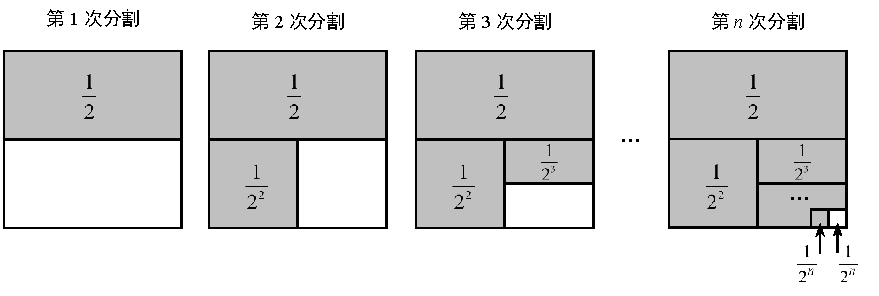
\includegraphics[width=0.8\linewidth]{23/2014a}
	\end{center}
	
	
	根据第$n$次分割图可得等式:${{\frac{{{1}}}{{{2}}}}{+}{\frac{{{1}}}{{{2}{^{{2}}}}}}{+}{\frac{{{1}}}{{{2}{^{{3}}}}}}{+}{\cdots 
		}{+}{\frac{{{1}}}{{{2}{^{{n}}}}}}}$=${{1}{-}{\frac{{{1}}}{{{2}{^{{n}}}}}}}$.
	
	\textbf{探究二:}计算${{\frac{{{1}}}{{{3}}}}{+}{\frac{{{1}}}{{{3}{^{{2}}}}}}{+}{\frac{{{1}}}{{{3}{^{{3}}}}}}{+}{\cdots 
		}{+}{\frac{{{1}}}{{{3}{^{{n}}}}}}}$.
	
	第1次分割,把正方形的面积三等分,其中阴影部分的面积为${{\frac{{{2}}}{{{3}}}}}$;
	
	第2次分割,把上次分割图中空白部分的面积继续三等分,阴影部分的面积之和为${{\frac{{{2}}}{{{3}}}}{+}{\frac{{{2}}}{{{3}{^{{2}}}}}}}$;
	
	第3次分割,把上次分割图中空白部分的面积继续三等分,{\ldots}{\ldots};
	
	{\ldots}{\ldots}
	
	第$n$次分割,把上次分割图中空白部分的面积最后三等分,所有阴影部分的面积之和为${{\frac{{{2}}}{{{3}}}}{+}{\frac{{{2}}}{{{3}{^{{2}}}}}}{+}{\frac{{{2}}}{{{3}{^{{3}}}}}}{+}{\cdots 
		}{+}{\frac{{{2}}}{{{3}{^{{n}}}}}}}$,最后空白部分的面积是${{\frac{{{1}}}{{{3}{^{{n}}}}}}}$.
	
	\begin{center}
		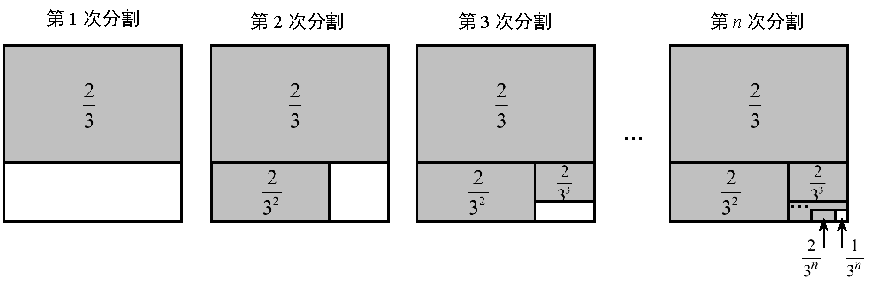
\includegraphics[width=0.8\linewidth]{23/2014b}
	\end{center}

	\begin{wrapfigure}{r}{0.2\linewidth}
		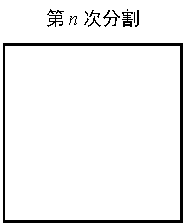
\includegraphics[width=\linewidth]{23/2014c}
		
		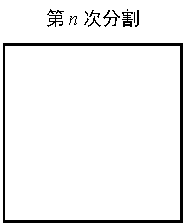
\includegraphics[width=\linewidth]{23/2014c}
	\end{wrapfigure}
	
	
	根据第$n$次分割图可得等式:${{\frac{{{2}}}{{{3}}}}{+}{\frac{{{2}}}{{{3}{^{{2}}}}}}{+}{\frac{{{2}}}{{{3}{^{{3}}}}}}{+}{\cdots 
		}{+}{\frac{{{2}}}{{{3}{^{{n}}}}}}}$=${{1}{-}{\frac{{{1}}}{{{3}{^{{n}}}}}}}$,
	
	两边同除以2, 
	得${{\frac{{{1}}}{{{3}}}}{+}{\frac{{{1}}}{{{3}{^{{2}}}}}}{+}{\frac{{{1}}}{{{3}{^{{3}}}}}}{+}{\cdots 
		}{+}{\frac{{{1}}}{{{3}{^{{n}}}}}}}$=${{\frac{{{1}}}{{{2}}}}{-}{\frac{{{1}}}{{{2}{\times 
					}{3}{^{{n}}}}}}}$.

	\textbf{探究三:}计算${{\frac{{{1}}}{{{4}}}}{+}{\frac{{{1}}}{{{4}{^{{2}}}}}}{+}{\frac{{{1}}}{{{4}{^{{3}}}}}}{+}{\cdots 
		}{+}{\frac{{{1}}}{{{4}{^{{n}}}}}}}$.
	
	(仿照上述方法,只画出第$n$次分割图,在图上标注阴影部分面积,并写出探究过程)
	
	\rule{0em}{8em}
	
	\textbf{解决问题:}计算${{\frac{{{1}}}{{{m}}}}{+}{\frac{{{1}}}{{{m}{^{{2}}}}}}{+}{\frac{{{1}}}{{{m}{^{{3}}}}}}{+}{\cdots 
		}{+}{\frac{{{1}}}{{{m}{^{{n}}}}}}}$.
	
	(只需画出第$n$次分割图,在图上标注阴影部分面积,并完成以下填空)
	
	根据第$n$次分割图可得等式:\ckong,
	
	所以,${{\frac{{{1}}}{{{m}}}}{+}{\frac{{{1}}}{{{m}{^{{2}}}}}}{+}{\frac{{{1}}}{{{m}{^{{3}}}}}}{+}{\cdots 
		}{+}{\frac{{{1}}}{{{m}{^{{n}}}}}}}=$\ckong.
	
	\textbf{拓广应用:}计算 
	${{\frac{{{5}{-}{1}}}{{{5}}}}{+}{\frac{{{5}{^{{2}}}{-}{1}}}{{{5}{^{{2}}}}}}{+}{\frac{{{5}{^{{3}}}{-}{1}}}{{{5}{^{{3}}}}}}{+}{\cdots 
		}{+}{\frac{{{5}{^{{n}}}{-}{1}}}{{{5}{^{{n}}}}}}}$\textbf{ 
		.}
	
	\rule{0em}{4em}
	
	\rule{0em}{4em}
	
	\nianfen{2013}在前面的学习中,我们通过对同一面积的不同表达和比较,根据图\textcircled{1}和图\textcircled{2}发现并验证了平方差公式和完全平方公式
	
	这种利用面积关系解决问题的方法,使抽象的数量关系因集合直观而形象化。
	
	\begin{center}
		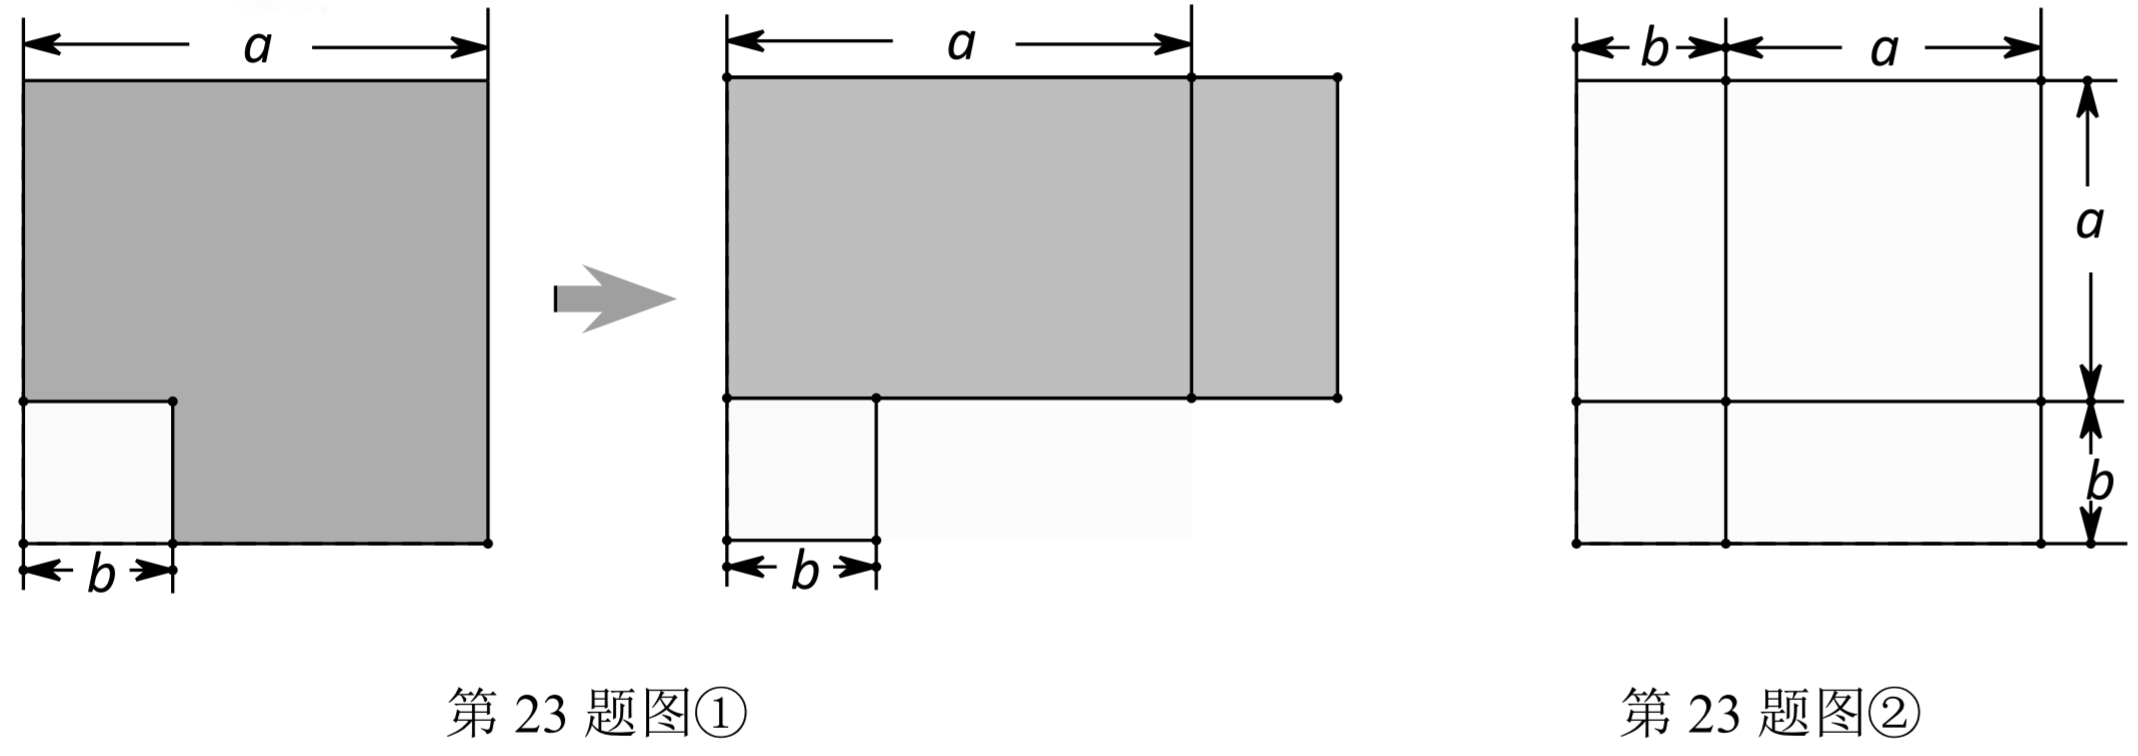
\includegraphics[width=0.9\linewidth]{23/2013a}
	\end{center}
	
	\textbf{【研究速算】}
	
	\begin{wrapfigure}{r}{0.35\linewidth}
			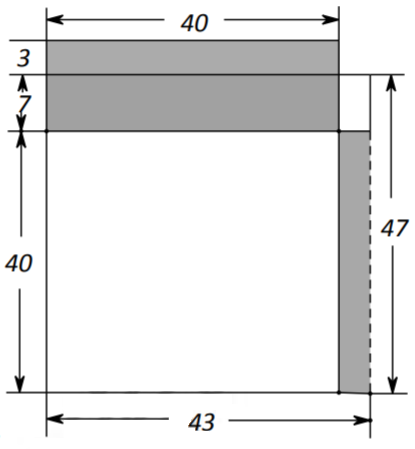
\includegraphics[width=\linewidth]{23/2013b}
	\end{wrapfigure}
	
	\textbf{提出问题:}47×43,56×54,79×71是一些十位数字相同,且个位数字之和是 10 的两个两位数相乘的算式,是否可以找到一种速算方法?
	
	\textbf{几何建模:}用矩形的面积表示两个正数的乘积,以 47×43 为例:
	
	(1)画长为 47,宽为 43 的矩形,如图\textcircled{3},将这个 47×43 的矩形从右边切下长 40,宽 3 的一条,拼接到原矩形的上面。
	
	(2)分析:原矩形面积可以有两种不同的表达方式,47×43
	的矩形面积或(40+7+3)×40 的矩形与右上角 3×7 的矩形
	面积之和,即 47×43=(40+10)×40+3×7=5×4×100+
	3×7=2021
	
	用文字表述 47×43 的速算方法是:十位数字 4 加 1 的和与 4 相乘,
	再乘以 100,加上个位数字 3 与 7 的积,构成运算结果
	
	\textbf{归纳提炼:}
	
	两个十位数字相同,并且个位数字之和是 10 的两位数相乘的速算方法是(用文字表述)
	
	\rule{0em}{6em}
	
	\begin{wrapfigure}{r}{0.4\linewidth}
			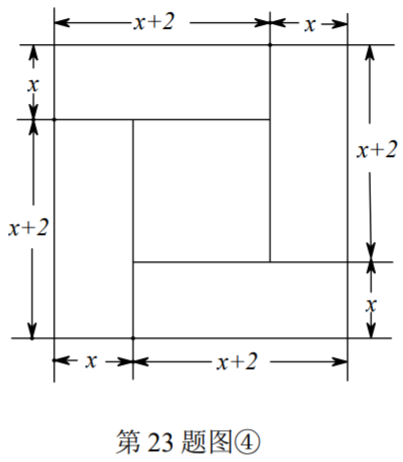
\includegraphics[width=\linewidth]{23/2013c}
	\end{wrapfigure}
	
	\textbf{【研究方程】}
	
	\textbf{提出问题:}怎么图解一元二次方程$x^2+2x-35=0(x>0)$?
	
	\textbf{几何建模:}
	
	(1)变形:$ x(x+2)=35 $
	
	(2)画四个长为$ x+2 $,宽为$ x $的矩形,构造图\textcircled{4}
	
	(3)分析:图中的大正方形面积可以有两种不同的表达方式,$ (x+x+2)^2 $或四个长$ x+2 $,宽$ x $的矩形之和,加上中间边长为 2 的小正方形面积
	
	即:$(x+x+2)^2=4x(x+2)+2^2$
	
	$\because x(x+2)=35$
	
	$\therefore (x+x+2)^2=4\times35+2^2$
	
	$\therefore (2x+2)^2=144$
	
	$\because x>0$
	
	$\therefore x=5$
	
	\textbf{归纳提炼:}求关于$ x $的一元二次方程$ x(x+b)=c(x>0,b>0,c>0) $的解
	
	要求参照上述研究方法,画出示意图,并写出几何建模步骤(用钢笔或圆珠笔画图,并标注相关线
	段的长)
	
	\rule{0em}{10em}\\
	
	\begin{wrapfigure}{r}{0.4\linewidth}
		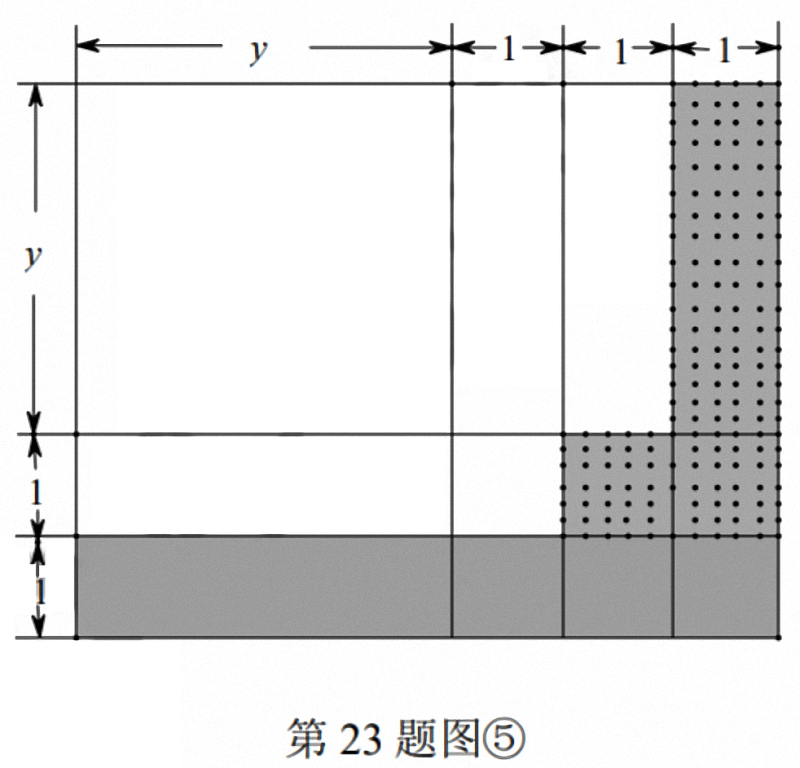
\includegraphics[width=\linewidth]{23/2013d}
	\end{wrapfigure}
	
	\textbf{【研究不等关系】}
	
	\textbf{提出问题:}怎么运用矩形面积表示$ (y+2)(y+3)与2y+5 $的大小关系(其中$ y>0 $)?
	
	\textbf{几何建模:}
	
	(1)画长$ y+3 $,宽$ y+2 $的矩形,按图\textcircled{5}方式分割
	
	(2)变形:$ 2y+5=(y+2)+(y+3) $
	
	(3)分析:图\textcircled{5}中大矩形的面积可以表示为$ (y+2)(y+3) $;阴影部分面积可以表示为$ (y+3)\times 1 $,
	
	画点部分的面积可表示为$ y+2 $,由图形的部分与整体的关系可知:$ (y+2)(y+3)>(y+2)+(y+3) $,即$ (y+2)(y+3)>2y+5 $
	
	\textbf{归纳提炼:}
	
	当$ a>2  $,$ b>2 $时,表示$ ab $与$ a+b $的大小关系
	
	根据题意,设$ a=2+m $,$ b=2+n(m>0,n>0) $,要求参照上述研究方法,画出示意图,并写出几何建模步骤(用钢笔或圆珠笔画图,并标注相关线段的长)
	
	\rule{0em}{6em}
	\clearpage
	
	\renewcommand{\nianfen}[1]{\hspace{-2em}{(#1\textbf{·}\textit{青岛}\textbf{·}24)}}
	\nianfen{2017}已知:Rt$ \triangle  EFP $ 和矩形 $ ABCD $ 如图\textcircled{1}摆放(点 $ P $ 与点 $ B $ 重合),点 $ F,B(P),C $ 在同一
	直线上,$ AB=EF=6 $ cm,$ BC=FP=8 $ cm,$ \angle EFP=90^{\circ}$.如图\textcircled{2},$ \triangle  EFP $从图\textcircled{1}的位置出发,沿 $ BC $ 方向匀速运动,速度为 1 cm/s,$ EP $ 与 $ AB $ 交于点 $ G $;同时,点 $ Q $ 从点 $ C $ 出发,沿 $ CD $
	方向匀速运动,速度为 1 cm/s.过点 $ Q $ 作 $ QM\perp  BD $,垂足为 $ H $,交 $ AD $ 于点 $ M $,连接 $ AF,PQ $.
	当点 $ Q $ 停止运动时,$ \triangle  EFP $ 也停止运动.设运动时间为 $ t $(s)$ (0<t<6) $,解答下列问题:
	
	(1)当 $ t $ 为何值时,$ PQ//BD $?
	
	(2)设五边形 $ AFPQM $ 的面积为 $ y $(cm$^2$),求 $ y $ 与 $ t $ 之间的函数关系式
	;
	(3)在运动过程中,是否存在某一时刻 $ t $,使 $ S $ 五边形 $ AFPQM:S_{\mbox{矩形}ABCD}=9:8$?若存在,求出 $ t $ 的值;若不存在,请说明理由;
	
	(4)在运动过程中,是否存在某一时刻 $ t $,使点 $ M $ 在线段 $ PG $ 的垂直平分线上?若存在,求出 $ t $ 的值;若不存在,请说明理由.
	
	\begin{center}
		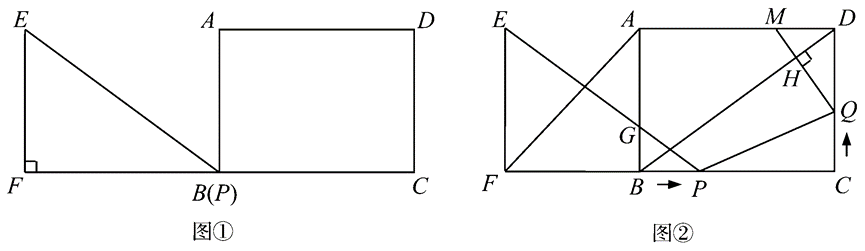
\includegraphics[width=0.9\linewidth]{24/2017}
	\end{center}

	\clearpage
	
	\nianfen{2016}已知:如图,在矩形 $ ABCD $ 中,$ AB=6$cm,$BC=8$cm,对角线 $ AC,BD $ 交于点 $ O $.点 $ P $ 从点 $ A $ 出发,沿 $ AD $ 方向匀速运动,速度为 $ 1 $cm/s;同时,点 $ Q $ 从点 $ D $ 出发,沿 $ DC $ 方向匀速运动,速度为 $ 1 $cm/s;当一个点停止运动时,另一个点也停止运动.连接 $ PO $ 并延长,交 $ BC $ 于点 $ E $,过点 $ Q $ 作 $ QF//AC $,交 $ BD $ 于点 $ F $.设运动时间为 $ t $(s)(0<t<6),解答下列问题:
	
	(1)当 $ t $ 为何值时,$ \triangle AOP $ 是等腰三角形?
	
	(2)设五边形 $ OECQF $ 的面积为 $ S $(cm$^2$),试确定 $ S $ 与 $ t $ 的函数关系式;
	
	(3)在运动过程中,是否存在某一时刻 $ t $,使 $ S_{\tiny\mbox{五边形}OECQF}:S_{\tiny\triangle ACD}=9:16 $?若存在,求出	$ t $ 的值;若不存在,请说明理由;
	
	(4)在运动过程中,是否存在某一时刻 $ t $,使 $ OD $ 平分$ \angle COP $?若存在,求出 $ t $ 的值;若不存在,请说明理由.
	
	\mbox{}\hfill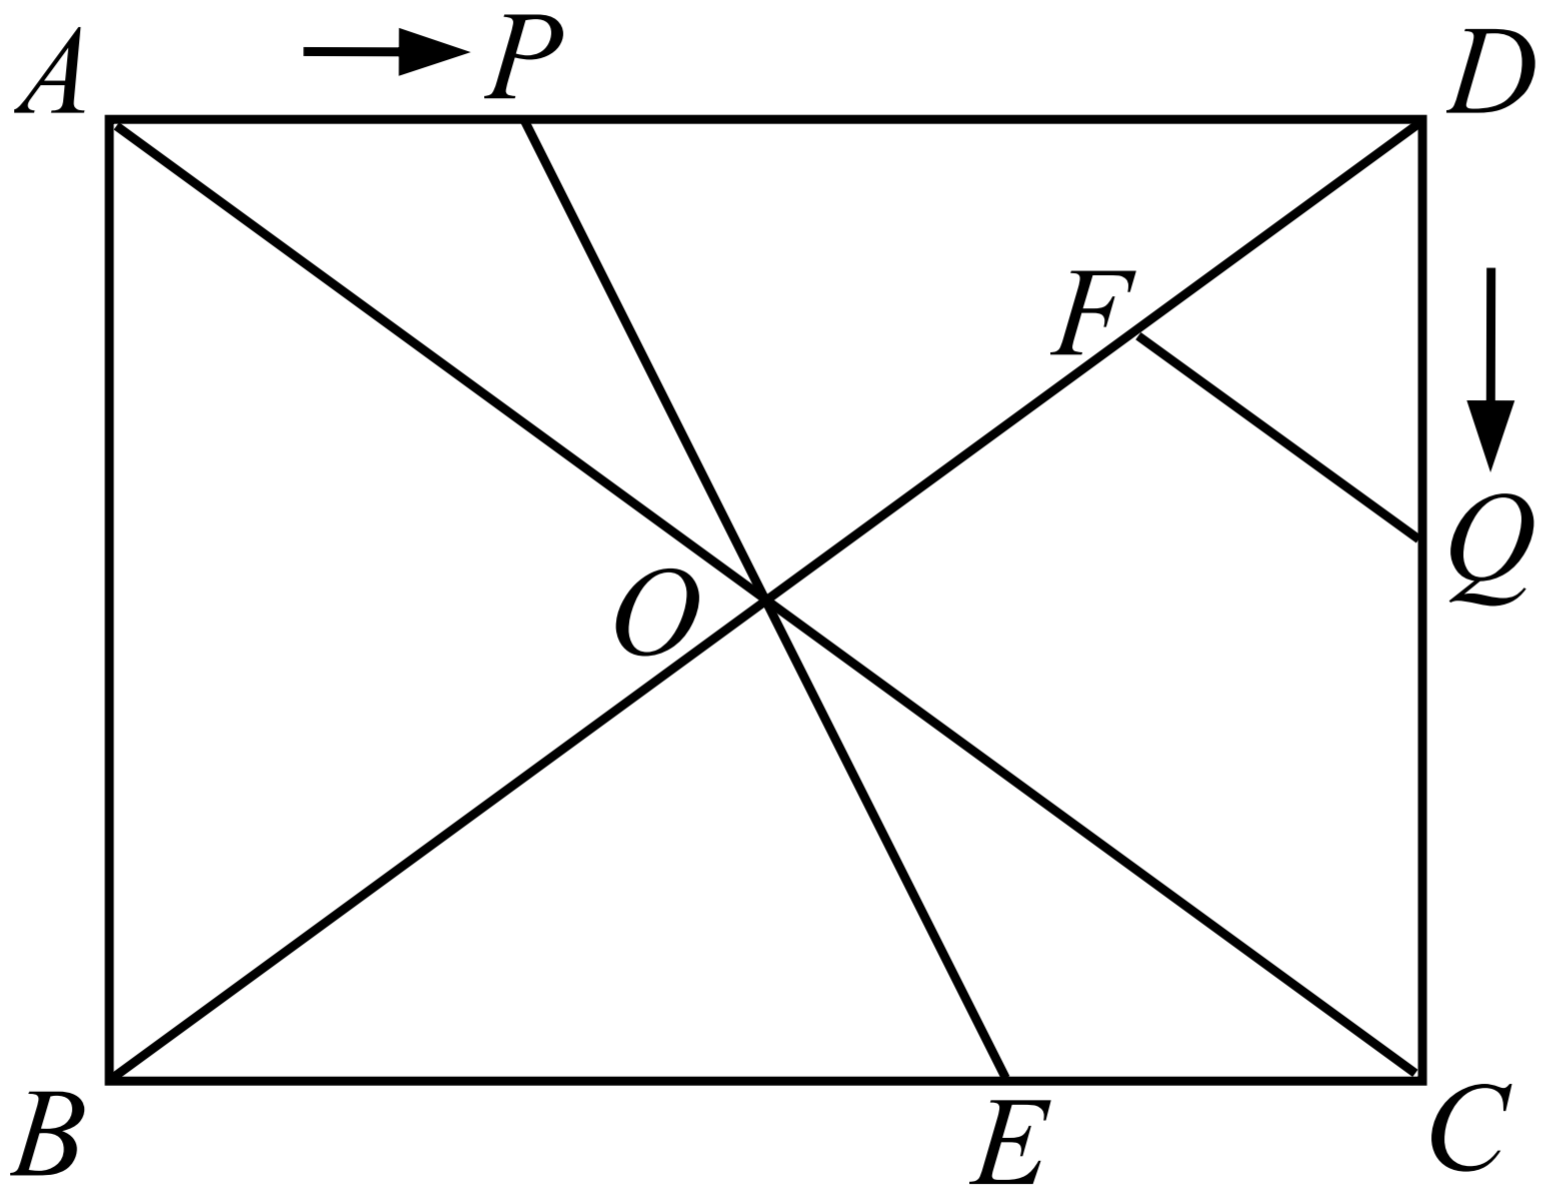
\includegraphics[width=0.3\linewidth]{24/2016}
	
	\clearpage
	
	\nianfen{2015}已知,如图\textcircled{1},在平行四边形$ ABCD $中,$ AB=3$cm,$BC=5$cm,$AC\perp AB,\triangle ACD $沿$ AC $的方向匀速平移得到$ \triangle PNM $,速度为1cm/s;同时,点$ Q $从点$ C $出发,沿$ CB $方向匀速移动,速度为1cm/s,当$ \triangle PNM $停止平移时,点$ Q $也停止移动,如图\textcircled{2},设移动时间为$ t $(s)(0<t<4),连接$ PQ,MQ,MC $,解答下列问题: 
	
	(1)当$ t $为何值时,$ PQ//MN $?
	
	(2)设$ \triangle QMC $的面积为y(cm$^2$),求$ y $与$ x $之间的函数关系式; 
	
	(3)是否存在某一时刻$ t $,使$ S_{\tiny\triangle QMC}:S_{\tiny\mbox{四边形}ABQP}=1:4 $?若存在,求出$ t $的值;若不存在,请说明理由.
	
	(4)是否存在某一时刻$ t $,使$ PQ\perp MQ $?若存在,求出$ t $的值;若不存在,请说明理由
	
	\begin{center}
		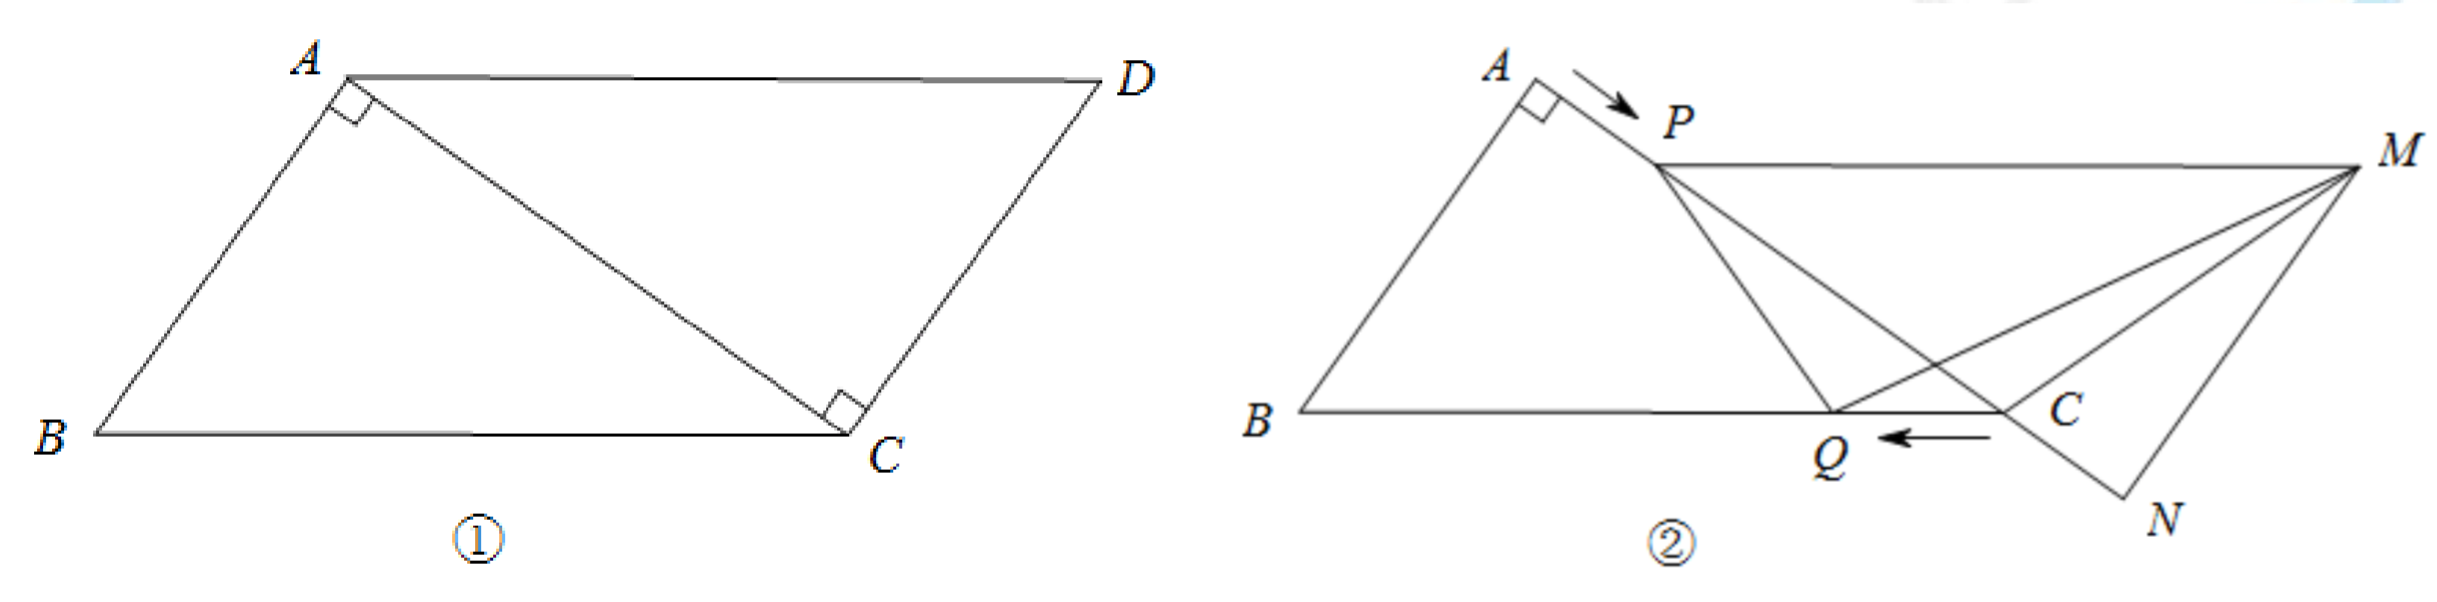
\includegraphics[width=0.8\linewidth]{24/2015}
	\end{center}
	
	
	
	\clearpage
	
	\nianfen{2014}已知:如图,菱形$ ABCD $中,对角线$ AC,BD $相交于点$ O $,且$ AC=12$cm,$BD=16$cm.点$ P $从点$ B $出发,沿$ BA $方向匀速运动,速度为1cm/s;同时,直线$ EF $从点$ D $出发,沿$ DB $方向匀速运动,速度为1cm/s,$ EF\perp BD $,且与$ AD,BD,CD $分别交于点$ E,Q,F $;当直线$ EF $停止运动时,点$ P $也停止运动.连接$ PF $,设运动时间为$ t $(s)(0<t<8).解答下列问题:
	
	(1)当$ t $为何值时,四边形$ APFD $是平行四边形?
	
	(2)设四边形$ APFE $的面积为$ y $(cm$^2$),求$ y $与$ t $之间的函数关系式;
	
	(3)是否存在某一时刻$ t $,使$ S_{\tiny\mbox{四边形}APFE}:S_{\tiny\mbox{菱形}ABCD}=17:4 $?若存在,求出$ t $的值,并求出此时$ P,E $两点间的距离;若不存在,请说明理由.
	
	\mbox{}\hfill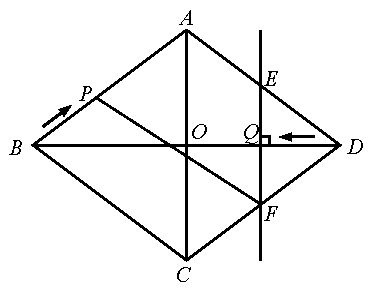
\includegraphics[width=0.4\linewidth]{24/2014}
	
	\clearpage
	
	\nianfen{2013}已知,如图,平行四边形$ ABCD  $中,$ AD=3$cm,$CD=1$cm,$ \angle B=45° $,点 $ P $ 从点 $ A $ 出发,沿 $ AD $ 方向匀速运动,速度为 3cm/s;点 $ Q $ 从点 $ C $ 出发,沿 $ CD $ 方向匀速运动,速度为 1cm/s,连接并延长 $ QP $ 交 $ BA $ 的延长线于点 $ M $,过 $ M $ 作 $ MN\perp BC $,垂足是 $ N $,设运动时间为 $ t $(s)(0<t<1),解答下列问题:
	
	(1)当 $ t $ 为何值时,四边形 $ AQDM $ 是平行四边形?
	
	(2)设四边形 $ ANPM $ 的面积为$ y $(cm$^2$),求 $ y $ 与 $ t $ 之间的函数关系式;
	
	(3)是否存在某一时刻 $ t $,使四边形 $ ANPM $ 的面积是平行四边形$ ABCD $ 面积的一半,若存在,求出相应的 $ t $ 值,若不存在,说明理由
	
	(4)连接 $ AC $,是否存在某一时刻 $ t $,使 $ NP $ 与 $ AC $ 的交点把线段 $ AC $ 分成$ 2:1 $的两部分?若存在,求出相应的 $ t $ 值,若不存在,说明理由
	
	\mbox{}\hfill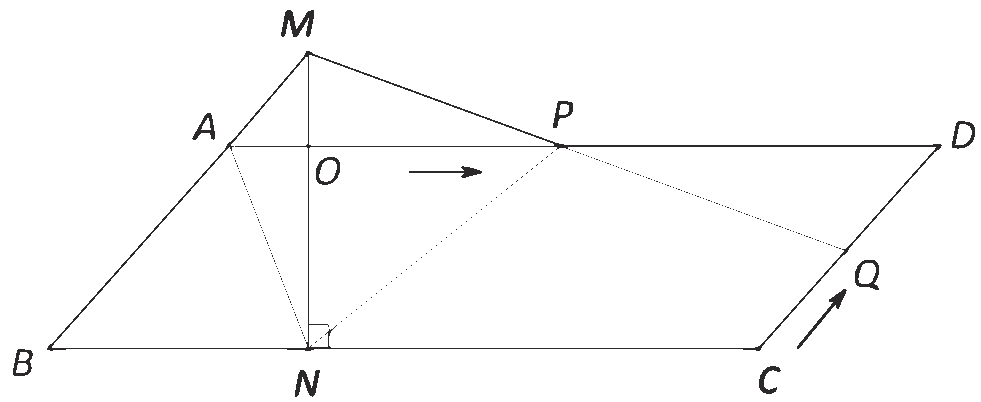
\includegraphics[width=0.5\linewidth]{24/2013}
	
\end{document}